\documentclass[10pt, oneside]{article}   	
\usepackage[left=25mm,top=25mm,right=25mm,bottom=25mm]{geometry}   
\geometry{a4paper}
\usepackage{algorithm,algpseudocode}  
\usepackage{graphicx}
\usepackage{tikz}
\usepackage{pgfplots}					
\usepackage{amssymb}
\usepackage{amsmath}
\usepackage{gensymb}
\usepackage{multirow}
\usepackage{url}
\usepackage{titlesec}
\usepackage{subcaption}
\usepackage[export]{adjustbox}
\usepackage[parfill]{parskip}
\usepackage{cite}
\usepackage{hyperref}
\usepackage{array}
\usepackage{siunitx}
\usepackage{listings}
\usepackage{fixltx2e}
\usepackage{color}
\usepackage{diagbox}
\usepackage[parfill]{parskip}
\setlength{\headsep}{5pt}
\graphicspath{ {images/} }
\lstset{
  basicstyle=\ttfamily,
  columns=fixed,
  fontadjust=true,
  basewidth=0.5em
}
\setcounter{topnumber}{3}
\setcounter{bottomnumber}{1}
\setcounter{totalnumber}{3}
\let\OLDthebibliography\thebibliography
\renewcommand\thebibliography[1]{
  \OLDthebibliography{#1}
  \setlength{\parskip}{0pt}
  \setlength{\itemsep}{1pt plus 0.5ex}
}
\renewcommand\thesection{\alph{section}}
\renewcommand\thesubsection{\thesection.\roman{subsection}}
\titleformat{\section}
{\normalfont\large\bfseries}{\thesection}{1em}{}
\titleformat{\subsection}
{\normalfont\normalsize\bfseries}{\thesubsection}{1em}{}
\title{\vspace{-1cm}Biomedical Information Processing (R214): main assignment report}
\author{Chongyang Shi \emph{(cs940)}}
\date{\today}							
\begin{document}
\maketitle

For the main course assignment, I am undertaking the second practical option (\textbf{1.2}): \emph{extracting chemical-disease associations from the biological literature}.

\section{Improving the Conditional Random Fields named entity recognizer}
\subsection{Ablating features from the original feature set} \label{subsec:ablating}

Based on the default \emph{n}-gram feature set in the feature extraction script, the script was modified to ablate each feature in turn. To provide a better understanding of the effects by offsets of surface form words, all surface forms of words within an offset of 1 (the trigram) were knocked out from the templates first, then just the surface forms of words before and after the current word (-1/1). Other features including the lemma, phonetic coding ($soundex$), part-of-speech, and chunk in IOB2 notation of the current word only. The resulting precisions, recall rates, and $F_1$-scores from ablating each feature on the \emph{devel} dataset are presented separately in Figures \ref{fig:ablation1}, \ref{fig:ablation2}, and \ref{fig:ablation3}. For each named entity class as well as the overall average, with none-ablated as reference, improved performance due to ablation are presented in \textbf{bold}.

\begin{figure}[h]
\begin{center}
\fontsize{9}{11}\selectfont
\begin{tabular}{|*{8}{c|}}\hline
\backslashbox{Class}{Ablated} & None & $word$ (all) & $word$ (-1/1) & $lemma$ & $soundex$ & $pos$ & $chunk$ \\ \hline
B-Chemical & 0.9178 & \textbf{0.9345} & \textbf{0.9409} & 0.9056 & 0.9015 & \textbf{0.9495} & \textbf{0.9210} \\ \hline
O                 & 0.9560 & 0.9471 & 0.9498 & 0.9540 & 0.9531 & 0.9499 & 0.9557 \\ \hline
B-Disease   & 0.8403 & 0.8242 & 0.8223 & \textbf{0.8418} & 0.8387 & \textbf{0.8412} & 0.8396 \\ \hline
I-Disease    & 0.7404 & 0.7152 & 0.7167 & \textbf{0.7467} & \textbf{0.7506} & \textbf{0.7631} & \textbf{0.7509} \\ \hline
I-Chemical  & 0.7556 & 0.6488 & 0.6745 & \textbf{0.7569} & \textbf{0.7612} & \textbf{0.7906} & \textbf{0.7682} \\ \hline
\textbf{Macro-average} & 0.8420 & 0.8142 & 0.8209 & 0.8410 & 0.8410 & \textbf{0.8589} &\textbf{ 0.8471} \\ \hline
\end{tabular}
\caption{\label{fig:ablation1} Resulting \textbf{precisions} on different named entity classes from ablating individual features from the original feature set. }
\end{center}
\end{figure}

\begin{figure}[h]
\begin{center}
\fontsize{9}{11}\selectfont
\begin{tabular}{|*{8}{c|}}\hline
\backslashbox{Class}{Ablated} & None & $word$ (all) & $word$ (-1/1) & $lemma$ & $soundex$ & $pos$ & $chunk$ \\ \hline
B-Chemical & 0.6664 & 0.5583 & 0.5955 & 0.6564 & 0.6520 & 0.5702 & 0.6652 \\ \hline
O                 & 0.9888 & 0.9888 & \textbf{0.9889} & 0.9888 & 0.9887 & \textbf{0.9908} & \textbf{0.9894} \\ \hline
B-Disease   & 0.6011 & 0.5514 & 0.5672 & 0.5669 & 0.5561 & 0.5806 & 0.5992 \\ \hline
I-Disease    & 0.6018 & 0.5530 & 0.5607 & 0.5993 & 0.5952 & \textbf{0.6029} & 0.5952 \\ \hline
I-Chemical  & 0.5961 & 0.5114 & 0.5275 & 0.5950 & 0.5910 & 0.5938 & \textbf{0.5990} \\ \hline
\textbf{Macro-average} & 0.6908 & 0.6326 & 0.6479 & 0.6813 & 0.6766 & 0.6677 & 0.6896 \\ \hline
\end{tabular}
\caption{\label{fig:ablation2} Resulting \textbf{recall rates} on different named entity classes from ablating individual features from the original feature set. }
\end{center}
\end{figure}

\begin{figure}[h]
\begin{center}
\fontsize{9}{11}\selectfont
\begin{tabular}{|*{8}{c|}}\hline
\backslashbox{Class}{Ablated} & None & $word$ (all) & $word$ (-1/1)& $lemma$ & $soundex$ & $pos$ & $chunk$ \\ \hline
B-Chemical & 0.7721 & 0.6992 & 0.7294 & 0.7611 & 0.7567 & 0.7125 & \textbf{0.7725} \\ \hline
O                 & 0.9721 & 0.9675 & 0.9690 & 0.9711 & 0.9706 & 0.9699 & \textbf{0.9723} \\ \hline
B-Disease   & 0.7008 & 0.6607 & 0.6713 & 0.6776 & 0.6687 & 0.6870 & 0.6993 \\ \hline
I-Disease    & 0.6640 & 0.6238 & 0.6292 & \textbf{0.6649} & 0.6639 & \textbf{0.6736} & \textbf{0.6641} \\ \hline
I-Chemical  & 0.6665 & 0.5720 & 0.5920 & 0.6662 & 0.6654 & \textbf{0.6782} & \textbf{0.6731} \\ \hline
\textbf{Macro-average} & 0.7551 & 0.7046 & 0.7182 & 0.7451 & 0.7451 & 0.7443 & \textbf{0.7562} \\ \hline
\end{tabular}
\caption{\label{fig:ablation3} Resulting \textbf{$F_1$-scores} on different named entity classes from ablating individual features from the original feature set.}
\end{center}
\end{figure}

Surprisingly, for chemicals at the beginning of entities (B-Chemcal), the precision (correct tags among those tagged) increased substantially when the surface form word feature is ablated. Ablating only the surface forms of before and after tokens (-1/1) produced slightly higher precision than ablating the entire surface form trigram. This is however accompanied by substantially reduced precisions on all other named entity classes, as well as reduced recall rate (correct tags among all relevant inputs that can be tagged) nearly across the board. As B-chemicals already bear a fairly high precision (91.78\%), it is not advisable to ablate the surface forms in exchange for lowering recall into the 50\%s. 

Ablation of the lemma (base word) and the phonetic coding ($soundex$) yielded minimal improvements to precisions on some named entity groups but minimal reductions on others. Recall rates all reduced by very small margins. Based on a generally negative outlook on the $F_1$-scores (combined metric of precision and recall), it is advisable not to alate either of he two features.

Ablating the part-of-speech produced the greatest precision improvements to most groups, but mostly lowered the recall rate substantially. This is also reflected in the overall negative outlook on the combined $F_1$-scores. Therefore it is not advisable to ablate the part-of-speech feature. 

Finally, ablating the chunk information from the feature set improved the precision without significantly affecting the recall rate in most cases, resulting in improved $F_1$-scores for all named entity classes barring diseases within entities (I-Disease) with a minimal decrease. Therefore, it is advisable to ablate the chunk information from the feature set used.

Vertically, precision and recall rates of terms outside entities (O) are high and only very minimally affected by ablating any of the features, which is generally expected in entity recognition operations due to the abundance of outside tokens between short named entities \cite{ratinov2009design}.

\subsection{Improvements to the base tagger}

After removing chunk information to improve performance of the base feature set (as described above), I will first experiment with expanding the \emph{n}-gram feature set by expanding unigram features into trigram features. Then, I will examine the effects of adjusting several parameters of the L-BFGS training algorithm used in \emph{crfsuite}.

\subsubsection{Expansion of unigram features}

Evaluations of word representation features in entity recognition by Tang et al. \cite{tang2014evaluating} demonstrated the benefits of using trigram features in word stemming. With this as inspiration, I iteratively expanded the unigram features of lemma, part-of-speech, and the phonetic coding ($soundex$) in the feature set. The order of expansion was chosen due to lemma being directly related to word stemming, part-of-speech correlations between neighbouring words normally being important, and the phonetic coding being the one left. The resulting performance information are shown in Figure \ref{fig:trigrams}.

\begin{figure}[h]
\begin{center}
\fontsize{9}{11}\selectfont
\begin{tabular}{|*{7}{c|}}\hline
\textbf{Expanded from unigram}  & \multicolumn{3}{c|}{None} & \multicolumn{3}{c|}{$lemma$}  \\ \hline 
\textbf{Entity Class} & Precision & Recall & $F_1$-score & Precision & Recall & $F_1$-score  \\ \hline
B-Chemical & 0.9210 & 0.6652 & 0.7725 & 0.9137 & 0.6695 & 0.7728 \\ \hline
O                 & 0.9557 & 0.9894 & 0.9723 & 0.9559 & 0.9890 & 0.9722\\ \hline
B-Disease   & 0.8396 & 0.5992 & 0.6993 & 0.8365 & 0.5992 & 0.6982 \\ \hline
I-Disease    & 0.7509 & 0.5952 & 0.6641 & 0.7519 & 0.6040 & 0.6699 \\ \hline
I-Chemical  & 0.7682 & 0.5990 & 0.6731 & 0.7820 & 0.6013 & 0.6798 \\ \hline
\textbf{Macro-average} & 0.8471 & 0.6896 & 0.7562 & 0.8480 & 0.6926 & 0.7586 \\ \hline \hline
\textbf{Expanded from unigram}  & \multicolumn{3}{c|}{$lemma$ + $pos$} & \multicolumn{3}{c|}{$lemma$ + $pos$ + $soundex$} \\ \hline 
\textbf{Entity Class} & Precision & Recall & $F_1$-score & Precision & Recall & $F_1$-score  \\ \hline
B-Chemical & 0.9077 & 0.6864 & 0.7817 & 0.9077 & 0.6875 & 0.7824 \\ \hline
O                 & 0.9574 & 0.9894 & 0.9731 & 0.9574 & 0.9894 & 0.9731 \\ \hline
B-Disease   & 0.8499 & 0.6162 & 0.7144 & 0.8477 & 0.6124 & 0.7111 \\ \hline
I-Disease    & 0.7819 & 0.6103 & 0.6855 & 0.7795 & 0.6110 & 0.6850 \\ \hline
I-Chemical  & 0.7884 & 0.6138 & 0.6903 & 0.8010 & 0.6241 & 0.7016 \\ \hline
\textbf{Macro-average} & 0.8570 & 0.7032 & 0.7690 & 0.8587 & 0.7049 & 0.7706 \\ \hline
\end{tabular}
\caption{\label{fig:trigrams} Resulting tagging performance on the \emph{devel} dataset after expanding unigram features into trigram features in the baseline feature set. ``None'' represents the baseline feature set with $chunk$ ablated.}
\end{center}
\end{figure}

While the precision of B-Chemical tagging continues to follow the declining trend discussed in \ref{subsec:ablating} (although not as severe in unigram expansion as in feature ablation), expanding unigram features of lemma, part-of-speech, and the phonetic coding into trigrams have resulted in improved or roughly equal precisions, recall rates -- and hence $F_1$-scores. Precision improvements were most notable from the additions of lemma and phonetic coding on chemicals within entities (I-Chemical), showing the influence of phonetic features of nearby entities on chemical entity recognition. The strongest improvement of recall and the $F_1$-score originated from expanding part-of-speech to nearby entities, demonstrating the importance of expanding the semantic scope. While precisions of some named entities took a small hit when the phonetic coding ($soundex$) was added, the improved macro-average precision as well as generally improved recall rates and $F_1$-scores were behind my choice of retaining all three unigram expansions.

\subsubsection{Adjustment of training parameters}

The L-BFGS training algorithm used in entity recognition uses L2 regularization, which is normally more efficient than L1 \cite{cortes20092}, with a regularization parameter influencing the levels of bias and overfitting. Various values around the default $c2 = 1$ were tested, with broadly similar trends in variations of precision, recall, and $F_1$-score in individual named entities. Therefore, only the macro-average metrics from tagging the \emph{devel} dataset with a model trained on each value of $c2$ are plotted in Figure \ref{fig:c2}.

 \begin{figure}[h]
\begin{center}
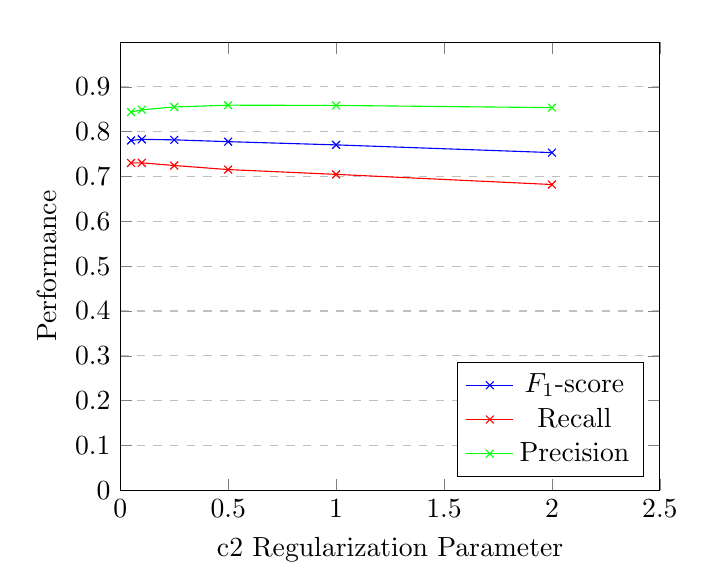
\begin{tikzpicture}
\begin{axis}[
    xlabel={c2 Regularization Parameter},
    ylabel={Performance},
    xmin=0, xmax=2.5,
    ymin=0, ymax=1.0,
    xtick={0, 0.5, ..., 2.5},
    ytick={0, 0.1, ..., 1.0},
    legend pos=south east,
    ymajorgrids=true,
    grid style=dashed,
]
 
\addplot[
color=blue,
mark=x,
]
coordinates {
(0.05,0.780505)(0.1,0.782937)(0.25,0.781873)(0.5,0.777822)(1.0,0.770645)(2.0,0.753415)
};
\addplot[
color=red,
mark=x,
]
coordinates {
(0.05,0.730290)(0.1,0.730579)(0.25,0.724635)(0.5,0.715561)(1.0,0.704877)(2.0,0.682223)
};
\addplot[
color=green,
mark=x,
]
coordinates {
(0.05,0.843873)(0.1,0.848921)(0.25,0.855177)(0.5,0.859233)(1.0,0.858653)(2.0,0.853710)
};
\legend{$F_1$-score,Recall,Precision}
\end{axis}
\end{tikzpicture}
\caption{\label{fig:c2} Resulting tagging performance on the \emph{devel} dataset with models trained on different c2 values.}
\end{center}
\end{figure}

A reduced $c2$ parameter results in longer training, but also generally improved recall and the overall $F_1$-score. With the adverse effects of extended training time and reduced precision (due to increased overfitting), as well as diminished gains in recall, $c2=0.25$ was chosen as the $c2$ value of choice.

With $c2=0.25$, L-BFGS also allows different line search algorithms, which yield roughly the same training speed, as well as almost the same performance with all named entity classes, as shown in Figure \ref{fig:linesearch}. Therefore the default More and Thuente's method is kept unchanged.

\begin{figure}[h]
\begin{center}
\fontsize{9}{11}\selectfont
\begin{tabular}{|*{10}{c|}}\hline
\textbf{Line Search}  & \multicolumn{3}{c|}{$MoreThuente$} & \multicolumn{3}{c|}{$Backtracking$} & \multicolumn{3}{c|}{$StrongBacktracking$}  \\ \hline 
\textbf{Entity Class} & Precision & Recall & $F_1$-score & Precision & Recall & $F_1$-score & Precision & Recall & $F_1$-score \\ \hline
B-Chemical & 0.9223 & 0.6972 & 0.7941 & 0.9223 & 0.6972 & 0.7941 & 0.9223 & 0.6972 & 0.7941 \\ \hline
O                 & 0.9609 & 0.9884 & 0.9745 & 0.9609 & 0.9884 & 0.9744 & 0.9609 & 0.9884 & 0.9744 \\ \hline
B-Disease   & 0.8363 & 0.6671 & 0.7422 & 0.8353 & 0.6656 & 0.7409 & 0.8352 & 0.6661 & 0.7411 \\ \hline
I-Disease    & 0.7515 & 0.6338 & 0.6876 & 0.7520 & 0.6330 & 0.6874 & 0.7520 & 0.6330 & 0.6874 \\ \hline
I-Chemical  & 0.8048 & 0.6367 & 0.7110 & 0.8048 & 0.6367 & 0.7110 & 0.8048 & 0.6367 & 0.7110 \\ \hline
\textbf{Macro-average} & 0.8552 & 0.7246 & 0.7819 & 0.8550 & 0.7242 & 0.7816 & 0.8550 & 0.7243 & 0.7816 \\ \hline
\end{tabular}
\caption{\label{fig:trigrams} Resulting tagging performance on the \emph{devel} dataset with different line search algorithms: More and Thuente's method, backtracking method with regular Wolfe condition, and backtracking method with strong Wolfe condition.}
\end{center}
\end{figure}



\bibliographystyle{IEEEtran}
\footnotesize{\bibliography{report}}
\end{document}  
